\documentclass[]{article}
\usepackage{lmodern}
\usepackage{amssymb,amsmath}
\usepackage{ifxetex,ifluatex}
\usepackage{fixltx2e} % provides \textsubscript
\ifnum 0\ifxetex 1\fi\ifluatex 1\fi=0 % if pdftex
  \usepackage[T1]{fontenc}
  \usepackage[utf8]{inputenc}
\else % if luatex or xelatex
  \ifxetex
    \usepackage{mathspec}
  \else
    \usepackage{fontspec}
  \fi
  \defaultfontfeatures{Ligatures=TeX,Scale=MatchLowercase}
\fi
% use upquote if available, for straight quotes in verbatim environments
\IfFileExists{upquote.sty}{\usepackage{upquote}}{}
% use microtype if available
\IfFileExists{microtype.sty}{%
\usepackage{microtype}
\UseMicrotypeSet[protrusion]{basicmath} % disable protrusion for tt fonts
}{}
\usepackage[margin=1in]{geometry}
\usepackage{hyperref}
\hypersetup{unicode=true,
            pdftitle={Assignment 3},
            pdfauthor={Terry Liu},
            pdfborder={0 0 0},
            breaklinks=true}
\urlstyle{same}  % don't use monospace font for urls
\usepackage{color}
\usepackage{fancyvrb}
\newcommand{\VerbBar}{|}
\newcommand{\VERB}{\Verb[commandchars=\\\{\}]}
\DefineVerbatimEnvironment{Highlighting}{Verbatim}{commandchars=\\\{\}}
% Add ',fontsize=\small' for more characters per line
\usepackage{framed}
\definecolor{shadecolor}{RGB}{248,248,248}
\newenvironment{Shaded}{\begin{snugshade}}{\end{snugshade}}
\newcommand{\KeywordTok}[1]{\textcolor[rgb]{0.13,0.29,0.53}{\textbf{#1}}}
\newcommand{\DataTypeTok}[1]{\textcolor[rgb]{0.13,0.29,0.53}{#1}}
\newcommand{\DecValTok}[1]{\textcolor[rgb]{0.00,0.00,0.81}{#1}}
\newcommand{\BaseNTok}[1]{\textcolor[rgb]{0.00,0.00,0.81}{#1}}
\newcommand{\FloatTok}[1]{\textcolor[rgb]{0.00,0.00,0.81}{#1}}
\newcommand{\ConstantTok}[1]{\textcolor[rgb]{0.00,0.00,0.00}{#1}}
\newcommand{\CharTok}[1]{\textcolor[rgb]{0.31,0.60,0.02}{#1}}
\newcommand{\SpecialCharTok}[1]{\textcolor[rgb]{0.00,0.00,0.00}{#1}}
\newcommand{\StringTok}[1]{\textcolor[rgb]{0.31,0.60,0.02}{#1}}
\newcommand{\VerbatimStringTok}[1]{\textcolor[rgb]{0.31,0.60,0.02}{#1}}
\newcommand{\SpecialStringTok}[1]{\textcolor[rgb]{0.31,0.60,0.02}{#1}}
\newcommand{\ImportTok}[1]{#1}
\newcommand{\CommentTok}[1]{\textcolor[rgb]{0.56,0.35,0.01}{\textit{#1}}}
\newcommand{\DocumentationTok}[1]{\textcolor[rgb]{0.56,0.35,0.01}{\textbf{\textit{#1}}}}
\newcommand{\AnnotationTok}[1]{\textcolor[rgb]{0.56,0.35,0.01}{\textbf{\textit{#1}}}}
\newcommand{\CommentVarTok}[1]{\textcolor[rgb]{0.56,0.35,0.01}{\textbf{\textit{#1}}}}
\newcommand{\OtherTok}[1]{\textcolor[rgb]{0.56,0.35,0.01}{#1}}
\newcommand{\FunctionTok}[1]{\textcolor[rgb]{0.00,0.00,0.00}{#1}}
\newcommand{\VariableTok}[1]{\textcolor[rgb]{0.00,0.00,0.00}{#1}}
\newcommand{\ControlFlowTok}[1]{\textcolor[rgb]{0.13,0.29,0.53}{\textbf{#1}}}
\newcommand{\OperatorTok}[1]{\textcolor[rgb]{0.81,0.36,0.00}{\textbf{#1}}}
\newcommand{\BuiltInTok}[1]{#1}
\newcommand{\ExtensionTok}[1]{#1}
\newcommand{\PreprocessorTok}[1]{\textcolor[rgb]{0.56,0.35,0.01}{\textit{#1}}}
\newcommand{\AttributeTok}[1]{\textcolor[rgb]{0.77,0.63,0.00}{#1}}
\newcommand{\RegionMarkerTok}[1]{#1}
\newcommand{\InformationTok}[1]{\textcolor[rgb]{0.56,0.35,0.01}{\textbf{\textit{#1}}}}
\newcommand{\WarningTok}[1]{\textcolor[rgb]{0.56,0.35,0.01}{\textbf{\textit{#1}}}}
\newcommand{\AlertTok}[1]{\textcolor[rgb]{0.94,0.16,0.16}{#1}}
\newcommand{\ErrorTok}[1]{\textcolor[rgb]{0.64,0.00,0.00}{\textbf{#1}}}
\newcommand{\NormalTok}[1]{#1}
\usepackage{longtable,booktabs}
\usepackage{graphicx,grffile}
\makeatletter
\def\maxwidth{\ifdim\Gin@nat@width>\linewidth\linewidth\else\Gin@nat@width\fi}
\def\maxheight{\ifdim\Gin@nat@height>\textheight\textheight\else\Gin@nat@height\fi}
\makeatother
% Scale images if necessary, so that they will not overflow the page
% margins by default, and it is still possible to overwrite the defaults
% using explicit options in \includegraphics[width, height, ...]{}
\setkeys{Gin}{width=\maxwidth,height=\maxheight,keepaspectratio}
\IfFileExists{parskip.sty}{%
\usepackage{parskip}
}{% else
\setlength{\parindent}{0pt}
\setlength{\parskip}{6pt plus 2pt minus 1pt}
}
\setlength{\emergencystretch}{3em}  % prevent overfull lines
\providecommand{\tightlist}{%
  \setlength{\itemsep}{0pt}\setlength{\parskip}{0pt}}
\setcounter{secnumdepth}{0}
% Redefines (sub)paragraphs to behave more like sections
\ifx\paragraph\undefined\else
\let\oldparagraph\paragraph
\renewcommand{\paragraph}[1]{\oldparagraph{#1}\mbox{}}
\fi
\ifx\subparagraph\undefined\else
\let\oldsubparagraph\subparagraph
\renewcommand{\subparagraph}[1]{\oldsubparagraph{#1}\mbox{}}
\fi

%%% Use protect on footnotes to avoid problems with footnotes in titles
\let\rmarkdownfootnote\footnote%
\def\footnote{\protect\rmarkdownfootnote}

%%% Change title format to be more compact
\usepackage{titling}

% Create subtitle command for use in maketitle
\newcommand{\subtitle}[1]{
  \posttitle{
    \begin{center}\large#1\end{center}
    }
}

\setlength{\droptitle}{-2em}

  \title{Assignment 3}
    \pretitle{\vspace{\droptitle}\centering\huge}
  \posttitle{\par}
    \author{Terry Liu}
    \preauthor{\centering\large\emph}
  \postauthor{\par}
    \date{}
    \predate{}\postdate{}
  

\begin{document}
\maketitle

\subsection{Question One}\label{question-one}

The datat file \textbf{Real-Estate.txt} contains information on the
homes sold in the Denver area during the yea 2003. The variables in this
data file are as follows:

\begin{longtable}[]{@{}ll@{}}
\toprule
Name & Representation\tabularnewline
\midrule
\endhead
Price & Selling price in \$1000\tabularnewline
Bedrooms & Number of bedrooms\tabularnewline
Size & Size of the home in square feet\tabularnewline
Pool & Swimming Pool(1=Yes,0=No)\tabularnewline
Distance & Distance from the home to the center of the
city\tabularnewline
Township & Township NO.\tabularnewline
Garage & Garage attached(1=Yes,0=No)\tabularnewline
Baths & Number of bathrooms\tabularnewline
\bottomrule
\end{longtable}

\subsubsection{Part A}\label{part-a}

Give a plot of selling price agaignst distance from the home to the
center of the city. Does there seem to be a relationship between the two
variables? If so, is the relationship direct or inverse ?

\subsubsection{Answer:}\label{answer}

\begin{Shaded}
\begin{Highlighting}[]
\NormalTok{data1 <-}\StringTok{ }\KeywordTok{read.table}\NormalTok{(}\StringTok{"Real-Estate.txt"}\NormalTok{,}\DataTypeTok{header=}\OtherTok{TRUE}\NormalTok{)}
\KeywordTok{names}\NormalTok{(data1)}
\end{Highlighting}
\end{Shaded}

\begin{verbatim}
## [1] "Price"    "Bedrooms" "Size"     "Pool"     "Distance" "Township"
## [7] "Garage"   "Baths"
\end{verbatim}

\begin{Shaded}
\begin{Highlighting}[]
\NormalTok{x <-}\StringTok{ }\NormalTok{data1}\OperatorTok{$}\NormalTok{Distance}
\NormalTok{y <-}\StringTok{ }\NormalTok{data1}\OperatorTok{$}\NormalTok{Price}

\KeywordTok{plot}\NormalTok{(x,y)}
\KeywordTok{abline}\NormalTok{(}\KeywordTok{lm}\NormalTok{(y}\OperatorTok{~}\NormalTok{x))}
\end{Highlighting}
\end{Shaded}

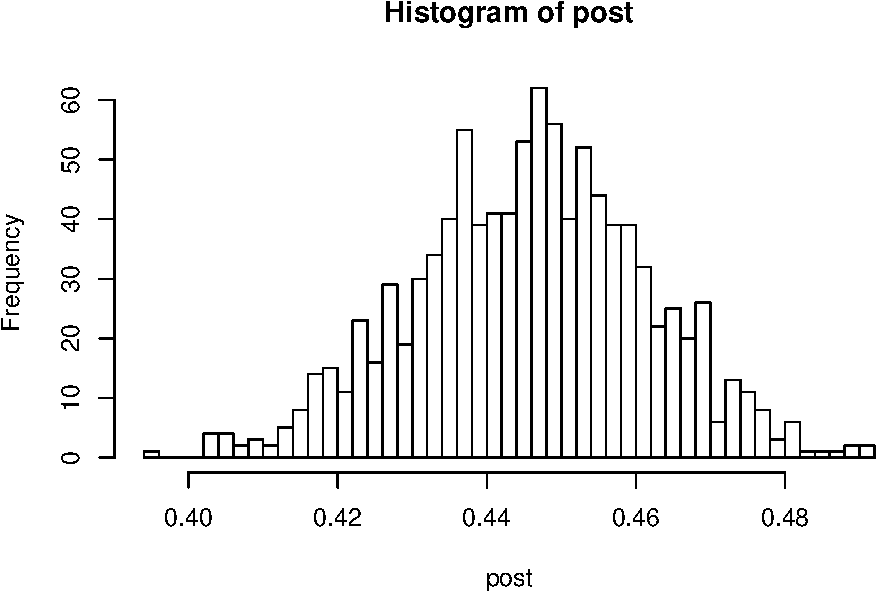
\includegraphics{Assignment_3_files/figure-latex/unnamed-chunk-1-1.pdf}
We can have the conclusion that there is negative relationship between
distance and the selling prze.

\subsubsection{Part B}\label{part-b}

Plot a histogram for selling price. Comment on the shape of the
distribution.

\begin{Shaded}
\begin{Highlighting}[]
\KeywordTok{hist.default}\NormalTok{(data1}\OperatorTok{$}\NormalTok{Price,}\DataTypeTok{xlim=}\KeywordTok{c}\NormalTok{(}\DecValTok{50}\NormalTok{,}\DecValTok{400}\NormalTok{),}\DataTypeTok{main=}\StringTok{'Price'}\NormalTok{)}
\end{Highlighting}
\end{Shaded}

\includegraphics{Assignment_3_files/figure-latex/unnamed-chunk-2-1.pdf}

\begin{Shaded}
\begin{Highlighting}[]
\NormalTok{skewness <-}\StringTok{ }\ControlFlowTok{function}\NormalTok{ (x, }\DataTypeTok{na.rm =} \OtherTok{FALSE}\NormalTok{) }

\NormalTok{\{}

  \ControlFlowTok{if}\NormalTok{ (na.rm) }

\NormalTok{    x <-}\StringTok{ }\NormalTok{x[}\OperatorTok{!}\KeywordTok{is.na}\NormalTok{(x)]}

  \KeywordTok{sum}\NormalTok{((x }\OperatorTok{-}\StringTok{ }\KeywordTok{mean}\NormalTok{(x))}\OperatorTok{^}\DecValTok{3}\NormalTok{)}\OperatorTok{/}\NormalTok{(}\KeywordTok{length}\NormalTok{(x) }\OperatorTok{*}\StringTok{ }\KeywordTok{sd}\NormalTok{(x)}\OperatorTok{^}\DecValTok{3}\NormalTok{)}

\NormalTok{\}}


\KeywordTok{skewness}\NormalTok{(data1}\OperatorTok{$}\NormalTok{Price)}
\end{Highlighting}
\end{Shaded}

\begin{verbatim}
## [1] 0.4605562
\end{verbatim}

We can get the skewness of these data (Selling Price) is equals to
\(0.4605562\), so, it is Positive Skew.

\subsubsection{Part C}\label{part-c}

Create a side-by-side box plots to compare the distribution of selling
price for homes with an attached garage and homes without a garage.
Comment on what you observe.

\begin{Shaded}
\begin{Highlighting}[]
\NormalTok{x_}\DecValTok{1}\NormalTok{ <-}\StringTok{ }\NormalTok{data1}\OperatorTok{$}\NormalTok{Price[data1}\OperatorTok{$}\NormalTok{Garage}\OperatorTok{==}\DecValTok{1}\NormalTok{]}
\NormalTok{x_}\DecValTok{2}\NormalTok{ <-}\StringTok{ }\NormalTok{data1}\OperatorTok{$}\NormalTok{Price[data1}\OperatorTok{$}\NormalTok{Garage}\OperatorTok{==}\DecValTok{0}\NormalTok{]}
\NormalTok{Garage <-}\StringTok{ }\KeywordTok{c}\NormalTok{(}\StringTok{"with Garage"}\NormalTok{,}\StringTok{"without Garage"}\NormalTok{)}
\KeywordTok{boxplot}\NormalTok{(x_}\DecValTok{1}\NormalTok{,x_}\DecValTok{2}\NormalTok{,}\DataTypeTok{names =}\NormalTok{ Garage, }\DataTypeTok{horizontal =} \OtherTok{TRUE}\NormalTok{, }\DataTypeTok{main =} \StringTok{"The Price comparison"}\NormalTok{,}\DataTypeTok{xlab=}\StringTok{"Price"}\NormalTok{)}
\end{Highlighting}
\end{Shaded}

\includegraphics{Assignment_3_files/figure-latex/unnamed-chunk-3-1.pdf}
Observation: The averge price of those have garage are higher than
without garage.

\subsubsection{Part D}\label{part-d}

There are five Townships in htis data. Draw a bar plot to compare the
number of homes sold in these Townships.

\begin{Shaded}
\begin{Highlighting}[]
\NormalTok{township_}\DecValTok{1}\NormalTok{ <-}\StringTok{ }\KeywordTok{length}\NormalTok{(data1}\OperatorTok{$}\NormalTok{Township[data1}\OperatorTok{$}\NormalTok{Township }\OperatorTok{==}\StringTok{ }\DecValTok{1}\NormalTok{])}
\NormalTok{township_}\DecValTok{2}\NormalTok{ <-}\StringTok{ }\KeywordTok{length}\NormalTok{(data1}\OperatorTok{$}\NormalTok{Township[data1}\OperatorTok{$}\NormalTok{Township }\OperatorTok{==}\StringTok{ }\DecValTok{2}\NormalTok{])}
\NormalTok{township_}\DecValTok{3}\NormalTok{ <-}\StringTok{ }\KeywordTok{length}\NormalTok{(data1}\OperatorTok{$}\NormalTok{Township[data1}\OperatorTok{$}\NormalTok{Township }\OperatorTok{==}\StringTok{ }\DecValTok{3}\NormalTok{])}
\NormalTok{township_}\DecValTok{4}\NormalTok{ <-}\StringTok{ }\KeywordTok{length}\NormalTok{(data1}\OperatorTok{$}\NormalTok{Township[data1}\OperatorTok{$}\NormalTok{Township }\OperatorTok{==}\StringTok{ }\DecValTok{4}\NormalTok{])}
\NormalTok{township_}\DecValTok{5}\NormalTok{ <-}\StringTok{ }\KeywordTok{length}\NormalTok{(data1}\OperatorTok{$}\NormalTok{Township[data1}\OperatorTok{$}\NormalTok{Township }\OperatorTok{==}\StringTok{ }\DecValTok{5}\NormalTok{])}

\NormalTok{name_township <-}\StringTok{ }\KeywordTok{c}\NormalTok{(}\StringTok{"township1"}\NormalTok{, }\StringTok{"township2"}\NormalTok{, }\StringTok{"township3"}\NormalTok{, }\StringTok{"township4"}\NormalTok{, }\StringTok{"township5"}\NormalTok{)}
\NormalTok{township <-}\StringTok{ }\KeywordTok{c}\NormalTok{(township_}\DecValTok{1}\NormalTok{, township_}\DecValTok{2}\NormalTok{, township_}\DecValTok{3}\NormalTok{ ,township_}\DecValTok{4}\NormalTok{, township_}\DecValTok{5}\NormalTok{)}
\NormalTok{tmp <-}\StringTok{ }\KeywordTok{as.vector}\NormalTok{(name_township)  }

\NormalTok{bar <-}\StringTok{ }\KeywordTok{barplot}\NormalTok{(township, }\DataTypeTok{axes=}\NormalTok{T, }\DataTypeTok{names =}\NormalTok{ name_township, }\DataTypeTok{las=}\DecValTok{2}\NormalTok{)}
\end{Highlighting}
\end{Shaded}

\includegraphics{Assignment_3_files/figure-latex/unnamed-chunk-4-1.pdf}

\begin{Shaded}
\begin{Highlighting}[]
\CommentTok{# axis(side = 1, lwd = 1, tck = -.015, labels = NA)}
\CommentTok{# # 添加x轴的坐标轴(包括坐标轴,刻度线和刻度线标签),但是却未显示刻度线标签}
\CommentTok{# axis(side = 2, lwd = 1, tck = -.015, labels = NA) # 添加y轴的坐标轴(包括坐标轴,刻度线和刻度线标签),但是却未显示刻度线标签}
\CommentTok{# axis(side = 1, lwd = 0, line = -.4) # 第二次添加x轴的坐标轴(包括坐标轴,刻度线和刻度线标签),但是只显示了刻度线标签(通过lwd = 0使坐标轴,刻度线未显示出来)}
\CommentTok{# axis(side = 2, lwd = 0, line = -.4, las = 1) # 第二次添加y轴的坐标轴(包括坐标轴,刻度线和刻度线标签),但是只显示了刻度线标签}
\end{Highlighting}
\end{Shaded}

\subsubsection{Part E}\label{part-e}

Draw a pie chart of the varialbe ``Baths'' and label the percentage of
each number of Bathrooms

\begin{Shaded}
\begin{Highlighting}[]
\NormalTok{x <-}\StringTok{ }\KeywordTok{c}\NormalTok{(}\KeywordTok{unique}\NormalTok{(data1}\OperatorTok{$}\NormalTok{Baths))}

\NormalTok{length_x <-}\StringTok{ }\KeywordTok{length}\NormalTok{(x)}



\NormalTok{lbls <-}\StringTok{ }\NormalTok{x}
\NormalTok{pct <-}\StringTok{ }\KeywordTok{round}\NormalTok{(x}\OperatorTok{/}\KeywordTok{sum}\NormalTok{(x)}\OperatorTok{*}\DecValTok{100}\NormalTok{)}
\NormalTok{lbls <-}\StringTok{ }\KeywordTok{paste}\NormalTok{(lbls, pct) }\CommentTok{# add percents to labels }
\NormalTok{lbls <-}\StringTok{ }\KeywordTok{paste}\NormalTok{(}\StringTok{"Baths="}\NormalTok{,lbls,}\StringTok{"%"}\NormalTok{,}\DataTypeTok{sep=}\StringTok{""}\NormalTok{) }\CommentTok{# ad % to labels }
\KeywordTok{pie}\NormalTok{(x,}\DataTypeTok{labels =}\NormalTok{ lbls, }\DataTypeTok{col=}\KeywordTok{rainbow}\NormalTok{(}\KeywordTok{length}\NormalTok{(lbls)),}
    \DataTypeTok{main=}\StringTok{"Pie Chart of Baths"}\NormalTok{)}
\end{Highlighting}
\end{Shaded}

\includegraphics{Assignment_3_files/figure-latex/unnamed-chunk-5-1.pdf}

\subsection{Question Two}\label{question-two}

Recently, it has been proposed that there is a non-linear relation
between the number of perople \(N\) in a city, and its economic output
per person \(Y\) (per captia \gross metropolitan product):
\[Y = y_0N^a + \text{ noise }\]

Using data from the 366 metropolitan area of the US (as of 2006) to
estimate \(a\), by minimizing the mean squared error,
\[\frac{1}{366} \sum_{i=1}^366 (Y_i - y_0N_i^a)^2\] over all a. We will
ess later in the class how we could estimate both parameters at onece,
but for now we'll treat \(y_0\) as know, and in particular equal =
\(6611\).


\end{document}
